%%%%%%%%%%%%%%%%%%%%%%%%%%%%%%%%%%%%%%%%%%%%%%%%%%%%%%%%%%%%%%%%%%%%%%
% Lớp 10 | Véctơ (chưa xét tọa độ) | Khái niệm véctơ
% Dạng 0H5?1-6: Toán thực tế  áp dụng véctơ
%%%%%%%%%%%%%%%%%%%%%%%%%%%%%%%%%%%%%%%%%%%%%%%%%%%%%%%%%%%%%%%%%%%%%%


% nguồn: TuLuan_Lop10_Dot2 (nhập 14/11/2026)
\begin{bt}%[0H5N1-6]%[Trong Nguyen]%[ma:d66da9dd]
	\immini
	{
		Quan sát ròng rọc hoạt động khi dùng lực để kéo một đầu của ròng rọc. 
		Chuyển động của đoạn dây mô tả bằng các vectơ $ \vec{a} $, $ \vec{b} $, $ 
		\vec{c} $ (như hình vẽ).
		\begin{enumerate}
			\item Hãy chỉ ra các vectơ cùng phương.
			\item Trong các vectơ đó, cho biết chúng cùng hướng hay ngược hướng.
		\end{enumerate}
	}
	{
		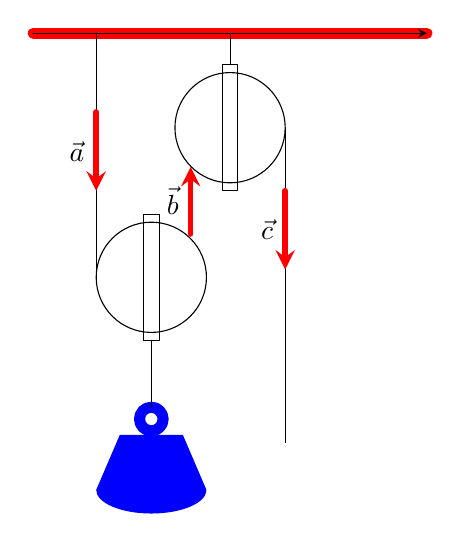
\begin{tikzpicture}[>=stealth,scale=1, line join = round, line cap 
			= round]
			\def \r{.8}
			;
			\coordinate (A) at (0,0);
			\coordinate (B) at (5,0);
			\coordinate (M) at (1.5,-3.1);
			\coordinate (N) at (2.5,-1.2);
			\coordinate (K) at (1.5-\r+0.1,0);
			\coordinate (H) at (2.5+\r-0.1,-1.2);
			\tikzset{truc/.pic={	\draw(-0.1,-\r) rectangle (0.1,\r);}}
			\draw 
			(M) pic[local bounding box=R1]
			{truc}
			(N) pic[local bounding box=R2]
			{truc};
			\tikzset{tron/.pic={	\draw (0,0) circle (\r-0.1);}}
			\draw 
			(M) pic[local bounding box=T1]
			{tron} 
			(N) pic[local bounding box=T2]
			{tron};
			\tikzset{can/.pic={
					\fill[blue](-0.4,0.4)--(-0.7,-0.3)--(-.7,-0.3) arc (-180:0:{0.7} and 
					{0.3})--(0.4,0.4)--cycle;
					\draw[line width=4,blue] (0,0.6) circle(0.15);
			}}
			\draw
			(1.5,-5.5) pic[local bounding box=C]
			{can};
			\draw[line width=4,red] (A)--(B);
			\draw[->] (A)--(B);
			\draw (R1)--(C) (R2)--(2.5,0) ;
			\draw (K)--++(-90:3.1);
			\draw (H)--++(-90:4);
			\draw[->,line width=2,red] (1.5-\r+0.1,-1)--++(-90:1) 
			node[midway,left,black] {$ \vec{a} $};
			\draw[->,line width=2,red] 
			(2.5+\r-0.1,-2)--++(-90:1)node[midway,left,black] 
			{$ \vec{c} $};
			\draw[->,line width=2,red] (2,-2.55)--++(90:.85)node[midway,left,black] {$ 
				\vec{b} $};
		\end{tikzpicture}
	}
	
	\loigiai{
		\begin{enumerate}
			\item Các vectơ cùng phương gồm: $ \vec{a} $, $ \vec{b} $, $ 
			\vec{c} $.
			\item Các vectơ cùng hướng gồm: $ \vec{a} $ và $ \vec{c} $. \\
			Các vectơ ngược hướng gồm: $ \vec{a} $ và $ \vec{b} $, $ \vec{b} $ 
			và $ \vec{c} $ . 
		\end{enumerate}
	}	
\end{bt}

% nguồn: TuLuan_Lop10_Dot2 (nhập 14/11/2026)
\begin{bt}%[0H5V1-6]%[ma:455f4b5c]
	Một vật $A$ được thả chìm hoàn toàn dưới đáy một cốc chất lỏng. Biết rằng trong ba cách biểu diễn lực đẩy Archimedes (Ác-si-mét) $\overrightarrow{F}$ và trọng lực $\overrightarrow{P}$ tác động lên vật $A$ ở hình dưới, có một cách biểu diễn đúng.
	\begin{center}
		\begin{tikzpicture}[scale=1, font=\footnotesize, line join=round, line cap=round, >=stealth]
			\begin{scope}[scale=.5]
				\draw[opacity=.15] (0,0) grid (26,6);
				\begin{scope}
					\path 
					(5,3) coordinate (A)
					;
					\fill[gray!40!white] ($(A)+(-160:1.45)$) rectangle ($(A)+(20:1.45)$);
					\draw (A)++(-90:.5)--++(180:2)--++(120:2.5);
					\draw (A)++(-90:.5)--++(0:2)--++(60:2.5);	
					\draw[->] (A)--+(-90:3) node[midway,right]{$\overrightarrow{P}$};
					\draw[->,line width=1.2pt] (A)--+(135:1.41) node[above]{$\overrightarrow{F}$};
					\foreach \p/\r in {A/180}
					\fill (\p) circle (1.5pt) node[shift={(\r:3mm)}]{$\p$};
					\node at ($(A)+(-90:4)$) {$a)$};
				\end{scope}
				\begin{scope}[xshift=8cm]
					\path 
					(5,3) coordinate (A)
					;
					\fill[gray!40!white] ($(A)+(-160:1.45)$) rectangle ($(A)+(20:1.45)$);
					\draw (A)++(-90:.5)--++(180:2)--++(120:2.5);
					\draw (A)++(-90:.5)--++(0:2)--++(60:2.5);	
					\draw[->] (A)--+(-90:3) node[midway,right]{$\overrightarrow{P}$};
					\draw[->,line width=1.2pt] (A)--+(90:1) node[above]{$\overrightarrow{F}$};
					\foreach \p/\r in {A/180}
					\fill (\p) circle (1.5pt) node[shift={(\r:3mm)}]{$\p$};
					\node at ($(A)+(-90:4)$) {$b)$};
				\end{scope}
				\begin{scope}[xshift=16cm]
					\path 
					(5,3) coordinate (A)
					;
					\fill[gray!40!white] ($(A)+(-160:1.45)$) rectangle ($(A)+(20:1.45)$);
					\draw (A)++(-90:.5)--++(180:2)--++(120:2.5);
					\draw (A)++(-90:.5)--++(0:2)--++(60:2.5);	
					\draw[->] (A)--+(-90:1) node[midway,below right]{$\overrightarrow{P}$};
					\draw[->,line width=1.2pt] (A)--+(90:3) node[midway,left]{$\overrightarrow{F}$};
					\foreach \p/\r in {A/180}
					\fill (\p) circle (1.5pt) node[shift={(\r:3mm)}]{$\p$};
					\node at ($(A)+(-90:4)$) {$c)$};
				\end{scope}
			\end{scope}
		\end{tikzpicture}
	\end{center}
	Hãy chỉ ra mối quan hệ giữa trọng lượng riêng của vật $A$ và trọng lượng riêng của chất lỏng trong cốc.
	\loigiai{
		Lực đẩy Archimedes và trọng lực đều tác động lên vật $A$ theo phương thẳng đứng, hai lực này có cùng phương nhưng ngược hướng. Do đó, hình a) không đúng. Vật $A$ chìm xuống đáy nên trọng lực $P$ (có hương từ trên xuống) lớn hơn lực đẩy Archimedes $F$ (có hướng từ dưới lên). Do vậy, hình c) không đúng.\\
		Vậy hình biểu diễn đúng là hình b). Theo đó, véc-tơ biểu diễn lực $\overrightarrow{P}$ có độ dài gấp $3$ lần độ dài của véc-tơ biểu diễn lực $\overrightarrow{F}$.\\
		Độ lớn của trọng lực và lực đẩy Archimedes tác động lên $A$ là $\left|\overrightarrow{P}\right|=d'\cdot V$, $\left|\overrightarrow{F}\right|=d\cdot V$, trong đó $V$ (m$^3$) là thể tích của vật $A$ và $d'$, $d$ (N/m$^3$) tương ứng là trọng lượng riêng của vật $A$ và của chất lỏng. Do $\left|\overrightarrow{P}\right|=3\left|\overrightarrow{F}\right|$ (theo hình b) nên $d'=3d$.Vậy trọng lượng riêng của vật $A$ gấp $3$ lần trọng lượng riêng của chất lỏng trong cốc.
	}
\end{bt}

% nguồn: TuLuan_Lop10_Dot2 (nhập 14/11/2026)
\begin{bt}%[0H5V1-6]%[ma:028eceba]
	Hai ca cô $A$ và $B$ chạy trên sông với các vận tốc riêng có cùng độ lớn là $15$ km/h. Tuy vậy, ca nô $A$ chạy xuôi dòng còn ca nô $B$ chạy ngược dòng. Vận tốc của dòng nước trên sông là $3$ km/h.
	\begin{enumerate}
		\item Hãy thể hiện trên hình vẽ, véc-tơ vận tốc $\overrightarrow{v}$ của dòng nước và các véc-tơ vận tốc thực tế $\overrightarrow{v}_a$, $\overrightarrow{v}_b$ của các ca nô $A$, $B$.
		\item Trong các véc-tơ $\overrightarrow{v}$, $\overrightarrow{v}_a$, $\overrightarrow{v}_b$, những cặp véc-tơ nào cùng phương và những cặp véc-tơ nào ngược hướng?
	\end{enumerate}
	\loigiai{
		\begin{enumerate}
			\item Độ lớn của véc-tơ vận tốc $\overrightarrow{v}$, $\overrightarrow{v}_a$, $\overrightarrow{v}_b$ tương ứng là $3$, $18$, $12$ (km/h). Do đó tỉ lệ độ dài giữa chúng là $\left|\overrightarrow{v}\right|: \left|\overrightarrow{v}_a\right|:\left|\overrightarrow{v}_b\right|=1:6:4$.
			\begin{center}
				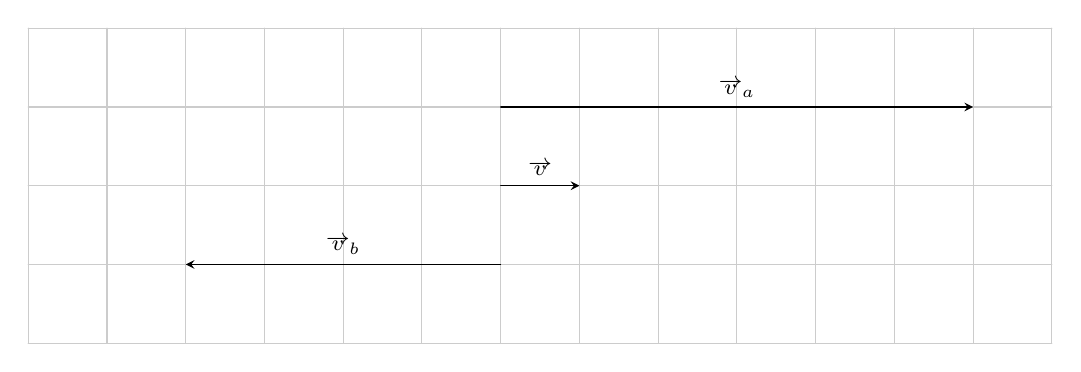
\begin{tikzpicture}[scale=1, font=\footnotesize, line join=round, line cap=round, >=stealth]
					\draw[opacity=.2] (0,0) grid (13,4);
					\draw[->] (6,1)--(2,1) node[midway,above]{$\overrightarrow{v}_b$};
					\draw[->] (6,2)--(7,2) node[midway,above]{$\overrightarrow{v}$};
					\draw[->] (6,3)--(12,3) node[midway,above]{$\overrightarrow{v}_a$};
				\end{tikzpicture}
			\end{center}
			\item Do ca nô $A$ chạy xuôi dòng nước nên các véc-tơ vận tốc $\overrightarrow{v}$ và $\overrightarrow{v}_a$ cùng phương và cùng hướng; do ca nô $B$ chạy ngược dòng nước, nên các véc-tơ $\overrightarrow{v}$ và $\overrightarrow{v}_b$ cùng phương và ngược hướng.\\
			Vậy trong các véc-tơ $\overrightarrow{v}$, $\overrightarrow{v}_a$, $\overrightarrow{v}_b$ có các cặp véc-tơ cùng phương là
			$\overrightarrow{v}$ và $\overrightarrow{v}_a$, $\overrightarrow{v}_a$ và $\overrightarrow{v}_b$, $\overrightarrow{v}_b$ và $\overrightarrow{v}$.\\
			Các cặp véc-tơ ngược hướng là $\overrightarrow{v}_a$ và $\overrightarrow{v}_b$, $\overrightarrow{v}_b$ và $\overrightarrow{v}$.
		\end{enumerate}
	}
\end{bt}

% nguồn: TuLuan_Lop10_Dot2 (nhập 14/11/2026)
\begin{bt}%[0H5V1-6]%[ma:7d05222c]
	\immini
	{
		Quan sát ròng rọc hoạt động khi dùng lực để kéo một đầu của ròng rọc. 
		Chuyển động của đoạn dây mô tả bằng các vectơ $ \overrightarrow{a} $, $ \overrightarrow{b} $, $ 
		\overrightarrow{c} $ (như hình vẽ).
		\begin{enumerate}
			\item Hãy chỉ ra các vectơ cùng phương.
			\item Trong các vectơ đó, cho biết chúng cùng hướng hay ngược hướng.
		\end{enumerate}
	}
	{
		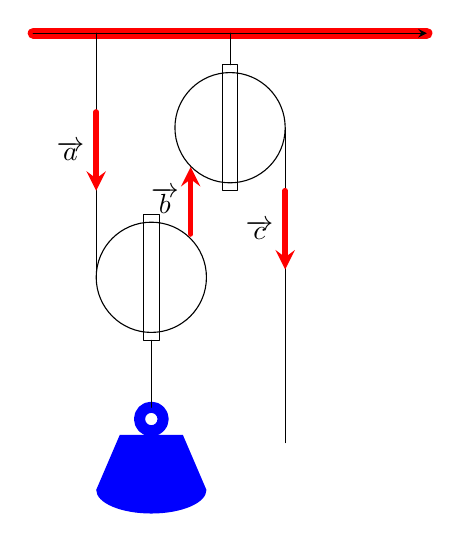
\begin{tikzpicture}[>=stealth,scale=1, line join = round, line cap 
			= round]
			\def \r{.8}
			;
			\coordinate (A) at (0,0);
			\coordinate (B) at (5,0);
			\coordinate (M) at (1.5,-3.1);
			\coordinate (N) at (2.5,-1.2);
			\coordinate (K) at (1.5-\r+0.1,0);
			\coordinate (H) at (2.5+\r-0.1,-1.2);
			\tikzset{truc/.pic={	\draw(-0.1,-\r) rectangle (0.1,\r);}}
			\draw 
			(M) pic[local bounding box=R1]
			{truc}
			(N) pic[local bounding box=R2]
			{truc};
			\tikzset{tron/.pic={	\draw (0,0) circle (\r-0.1);}}
			\draw 
			(M) pic[local bounding box=T1]
			{tron} 
			(N) pic[local bounding box=T2]
			{tron};
			\tikzset{can/.pic={
					\fill[blue](-0.4,0.4)--(-0.7,-0.3)--(-.7,-0.3) arc (-180:0:{0.7} and 
					{0.3})--(0.4,0.4)--cycle;
					\draw[line width=4,blue] (0,0.6) circle(0.15);
			}}
			\draw
			(1.5,-5.5) pic[local bounding box=C]
			{can};
			\draw[line width=4,red] (A)--(B);
			\draw[->] (A)--(B);
			\draw (R1)--(C) (R2)--(2.5,0) ;
			\draw (K)--++(-90:3.1);
			\draw (H)--++(-90:4);
			\draw[->,line width=2,red] (1.5-\r+0.1,-1)--++(-90:1) 
			node[midway,left,black] {$ \overrightarrow{a} $};
			\draw[->,line width=2,red] 
			(2.5+\r-0.1,-2)--++(-90:1)node[midway,left,black] 
			{$ \overrightarrow{c} $};
			\draw[->,line width=2,red] (2,-2.55)--++(90:.85)node[midway,left,black] {$ 
				\overrightarrow{b} $};
		\end{tikzpicture}
	}
	
	\loigiai{
		\begin{enumerate}
			\item Các vectơ cùng phương gồm: $ \overrightarrow{a} $, $ \overrightarrow{b} $, $ 
			\overrightarrow{c} $.
			\item Các vectơ cùng hướng gồm: $ \overrightarrow{a} $ và $ \overrightarrow{c} $. \\
			Các vectơ ngược hướng gồm: $ \overrightarrow{a} $ và $ \overrightarrow{b} $, $ \overrightarrow{b} $ 
			và $ \overrightarrow{c} $ . 
		\end{enumerate}
	}	
\end{bt}
